\documentclass{beamer}
\usepackage{beamerthemesplit}
\usepackage{wrapfig}
\usetheme{SPbGU}
\usepackage{pdfpages}
\usepackage{amsmath}
\usepackage{cmap} 
\usepackage[T2A]{fontenc} 
\usepackage[utf8]{inputenc}
\usepackage[english,russian]{babel}
\usepackage{indentfirst}
\usepackage{amsmath}
\usepackage{tikz}
\usepackage{multirow}
\usepackage[noend]{algpseudocode}
\usepackage{algorithm}
\usepackage{algorithmicx}
\usetikzlibrary{shapes,arrows}
\usepackage{fancyvrb}
\newtheorem{rutheorem}{Теорема}
\newtheorem{ruproof}{Доказательство}
\newtheorem{rudefinition}{Определение}
\newtheorem{rulemma}{Лемма}
\beamertemplatenavigationsymbolsempty

\title[]{Синтаксический анализ регулярных множеств}
\subtitle[]{В рамках проекта лаборатории JetBrains}
\institute[СПбГУ]{
Санкт-Петербургский государственный университет \\
Кафедра системного программирования }

\author[Вербицкая Екатерина]{Вербицкая Екатерина Андреевна, 544 группа \\
  \and  
    {\bfseries Научный руководитель:} ст.пр. С.В. Григорьев \\ 
  \and
    {\bfseries Рецензент:} программист "ИнтеллиДжей Лабс" А.А. Бреслав }

\date{18 июня 2015г.}

\definecolor{orange}{RGB}{179,36,31}

\begin{document}
{

\begin{frame}
  \begin{center}
  {
\includegraphics[width=1cm]{SPbGU_Logo.png}}
  \end{center}
  \titlepage
\end{frame}
}

\begin{frame}[fragile]
  \transwipe[direction=90]
  \frametitle{Встроенные выражения}
  \begin{itemize}
    \item Динамический SQL
      \begin{Verbatim}[commandchars=\\\{\}]
\textcolor{blue}{IF} @X = @Y
    \textcolor{blue}{SET} @TBL = \textcolor{orange}{' #table1 '}
\textcolor{blue}{ELSE}
    \textcolor{blue}{SET} @TBL = \textcolor{orange}{' table2 '}
\textcolor{blue}{SET} @S = \textcolor{orange}{'SELECT x FROM'} + @TBL + \textcolor{orange}{'WHERE ISNULL(n,0) > 1'}
EXECUTE (@S)
       \end{Verbatim}
    \item Встроенный SQL
      \begin{Verbatim}[commandchars=\\\{\}]
\textcolor{blue}{SqlCommand} myCommand = new \textcolor{blue}{SqlCommand}(
    \textcolor{orange}{"SELECT * FROM table WHERE Column = @Param2"},
    myConnection);
myCommand.Parameters.Add(myParam2);
      \end{Verbatim}
    \end{itemize}
\end{frame}




\begin{frame}[fragile]
\transwipe[direction=90]
\frametitle{Схема анализа встроенного кода}
\begin{tabular}{p{6cm}|p{6cm}}
Фрагмент кода & Регулярная аппроксимация
\\
\begin{minipage}{3in}
  \begin{Verbatim}[commandchars=\\\{\}]

\textcolor{blue}{string} res = \textcolor{orange}{""};
\textcolor{blue}{for}(i = 0; i < l; i++) \{
    res = \textcolor{orange}{"()"} + res;
\}   

  \end{Verbatim}
\end{minipage}
& 
\begin{minipage}{1in}
  \begin{Verbatim}[commandchars=\\\{\}]
(\textcolor{orange}{"()"})*
  \end{Verbatim} 
\end{minipage}
\\ \hline 
Множество значений
&
Граф конечного автомата
\\
\begin{minipage}{1in}
  \begin{Verbatim}[commandchars=\\\{\}]

\{\textcolor{orange}{""},
 \textcolor{orange}{"()"},
 \textcolor{orange}{"()()"},
 ...
 \textcolor{orange}{"()"}^l,
\}
  \end{Verbatim}
\end{minipage}
&
\\
&
\multirow{-8}*{\!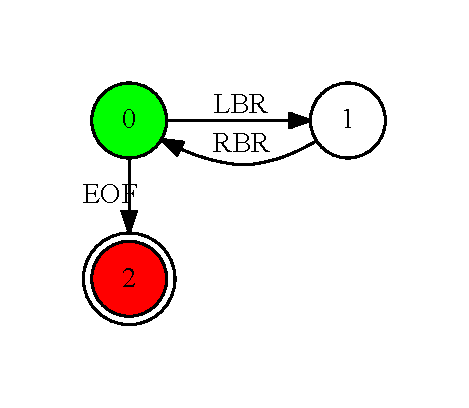
\includegraphics[width=5cm]{pictures/in3.pdf}}
\\
\end{tabular}
\end{frame}

\begin{frame}
  \transwipe[direction=90]
  \frametitle{Существующие инструменты}
  \begin{itemize}
    \item Java String Analyzer, Alvor
    \begin{itemize}
      \item Регулярная аппроксимация
    \end{itemize}
    \item PHP String Analyzer
    \begin{itemize}
      \item КС-аппроксимация
    \end{itemize}
    \item Kyung-Goo Doh et al.
    \begin{itemize}
      \item Решение уравнений потока данных над множеством LR-стеков
    \end{itemize}
  \end{itemize}
  
  \begin{itemize}
    \item Недостатки
    \begin{itemize}
      \item Плохо расширяемы
      \item Не строят структурного представления кода
    \end{itemize}
  \end{itemize}
\end{frame}

\begin{frame}
  \transwipe[direction=90]
  \frametitle{Постановка задачи}
  \textbf{Целью} работы является разработка алгоритма, применимого для синтаксического 
анализа встроенных языков
  
  \textbf{Задачи}:
  \begin{itemize}
    \item Разработать алгоритм синтаксического анализа регулярной аппроксимации динамически формируемых строковых выражений, строящий конечное представление леса разбора
    \item Доказать корректность алгоритма
    \item Реализовать предложенный алгоритм
    \item Провести апробацию
  \end{itemize}
\end{frame}
            
\begin{frame}
  \transwipe[direction=90]
  \frametitle{Алгоритм}
  \begin{itemize}
    \item \textbf{Вход}: эталонная ДКС-грамматика $G$ и граф ДКА без 
$\epsilon$-переходов над алфавитом терминалов $G$
    \item \textbf{Выход}: конечное представление множества деревьев, соответствующих 
всем корректным цепочкам, принимаемым входным автоматом
  \end{itemize}
\end{frame}

\begin{frame}[fragile]
\transwipe[direction=90]
\frametitle{Алгоритм}
\begin{tabular}{p{5cm} p{7cm}}
\begin{minipage}{3in}
  \begin{Verbatim}[commandchars=\\\{\}]

\textcolor{blue}{string} res = \textcolor{orange}{""};
\textcolor{blue}{for}(i = 0; i < l; i++) \{
    res = \textcolor{orange}{"()"} + res;
\}   

  \end{Verbatim}
\end{minipage}
&
Результат (SPPF):
\\
Аппроксимация: 
&
\multirow{-2}*{\!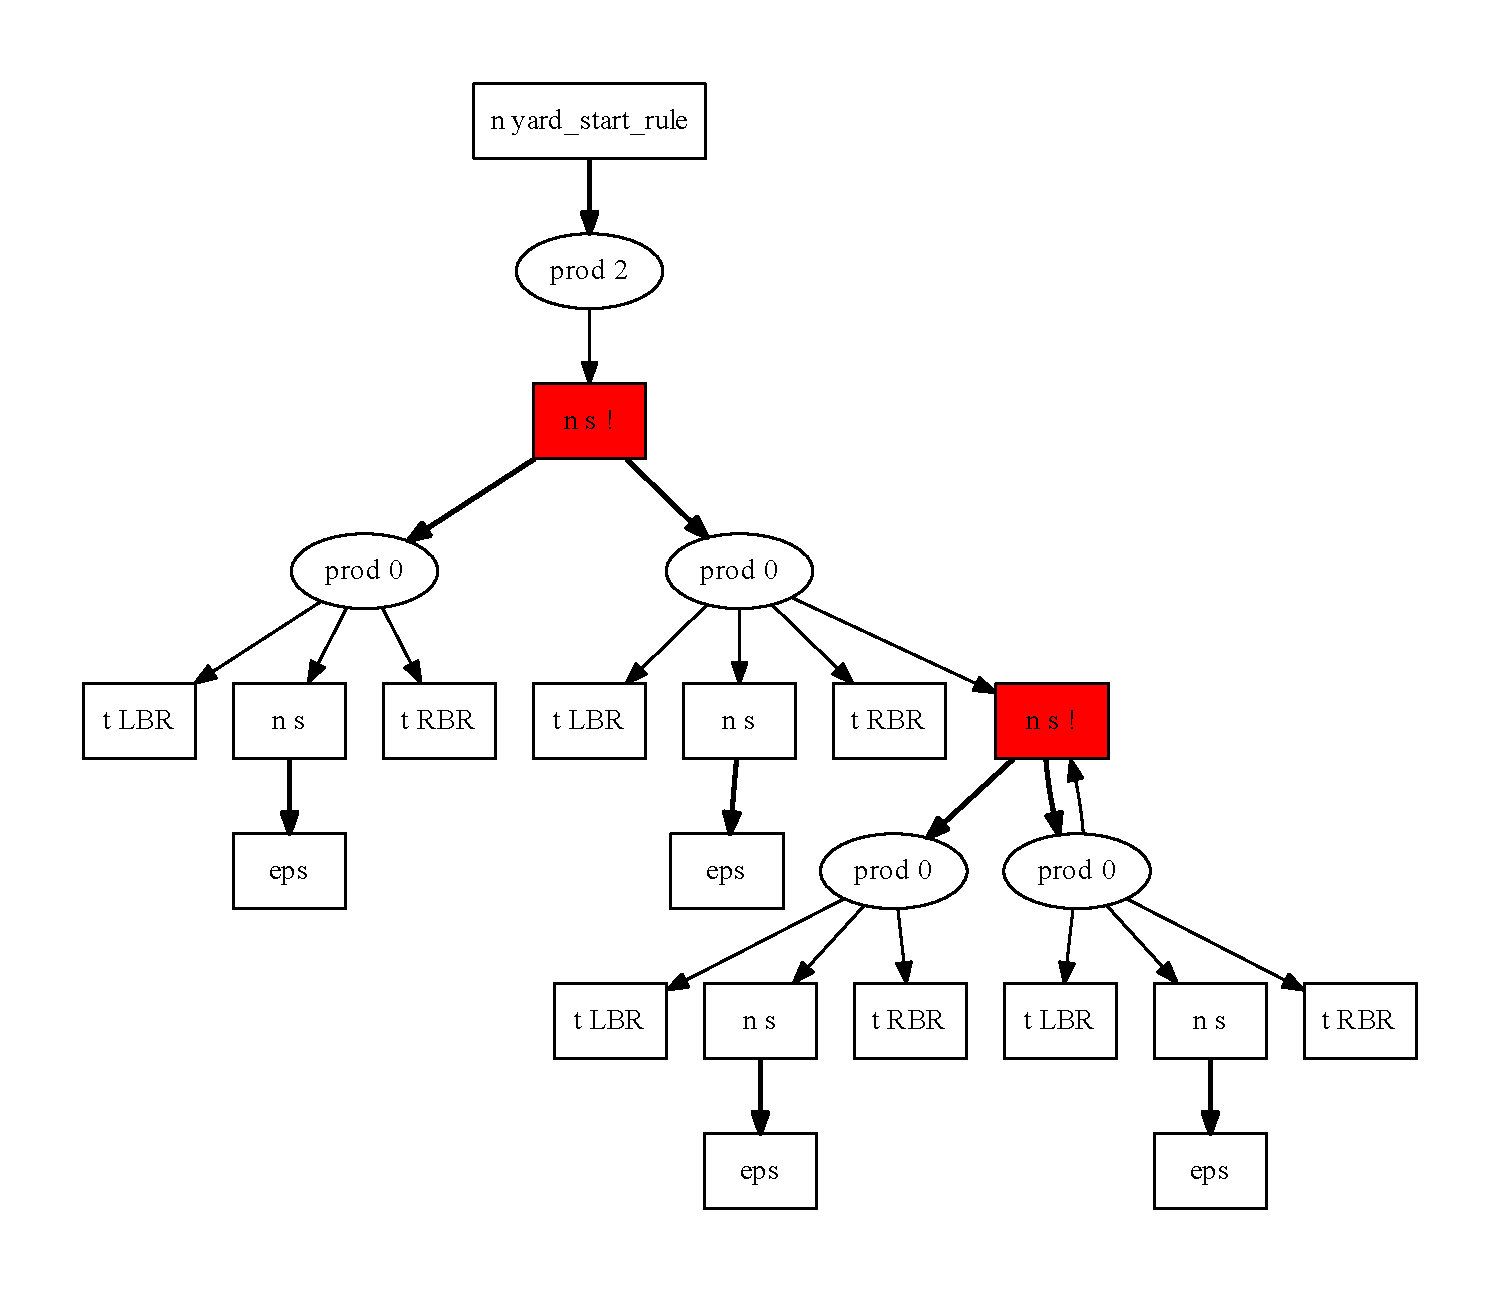
\includegraphics[width=6.8cm]{pictures/out3.pdf}}
\\
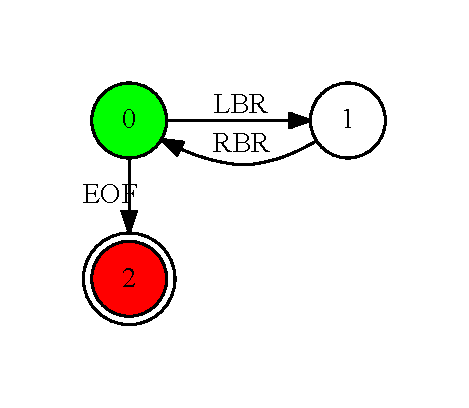
\includegraphics[width=3cm]{pictures/in3.pdf}
&
\\      
Грамматика: &
\\
\vspace{-20pt}
$$
\begin{array}{crcl}
&start &::=& s \\
&s & ::= & \mbox{\texttt{LBR }} s \mbox{\texttt{ RBR }} s\\
&s & ::= &\epsilon
\end{array}
$$
& 
\end{tabular}
\end{frame}

\begin{frame}
  \transwipe[direction=90]
  \frametitle{Алгоритм}
  \begin{itemize}
    \item Управление стеком и построение леса разбора (SPPF) осуществляется, 
как в RNGLR-алгоритме
    \item С каждой вершиной входного графа ассоциируется множество LR-состояний синтаксического анализатора
    \item Последовательное построение стека GSS во время обхода входного графа
    \item Для управления порядком обработки вершин входного графа используется 
очередь. Вершина добавляется в очередь, когда в GSS добавляется новое ребро с 
концом в этой вершине
  \end{itemize}
\end{frame}

\begin{frame}
\transwipe[direction=90]
\frametitle{Алгоритм: корректность}
\begin{tabular}{p{5.3cm} p{6.7cm}}
\emph{Корректное дерево} -- дерево вывода цепочки, накопленной вдоль некоторого 
пути в графе
&
\\
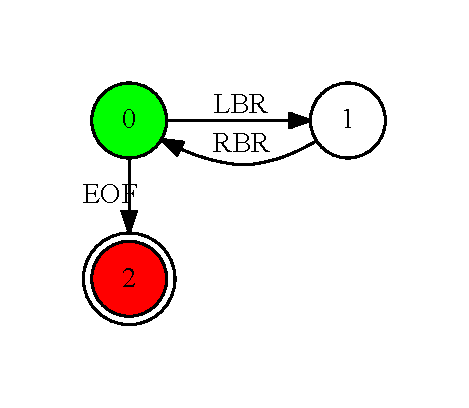
\includegraphics[width=5cm]{pictures/in3.pdf}
&
\includegraphics[width=6cm]{pictures/sppf2.eps}
\end{tabular}
\end{frame}


\begin{frame}
  \transwipe[direction=90]
  \frametitle{Алгоритм: корректность}
  \begin{rutheorem}[Завершаемость]
    Алгоритм завершается для любой ДКС-грамматики $G$ и любого ДКА без $\epsilon-$переходов.
  \end{rutheorem}
  
  \begin{rutheorem}[Корректность]
    Любое дерево, извлечённое из SPPF, корректно.
  \end{rutheorem}

  \begin{rutheorem}[Корректность]
    Для строки, сооответствующей любому пути $p$ во входном графе, имеющей вывод в эталонной грамматике $G$, корректное дерево, соответствующее $p$, может быть извлечено из SPPF.
  \end{rutheorem}
\end{frame}

\begin{frame}
  \transwipe[direction=90]
  \frametitle{Реализация}
  \begin{itemize}
    \item Алгоритм реализован как часть проекта YaccConstructor на~языке~F\#
    \item Переиспользован генератор RNGLR-таблиц и структуры данных GSS и SPPF
    \begin{itemize}
      \item Дипломная работа выпускника кафедры системного программирования 
Авдюхина Дмитрия
    \end{itemize}
  \end{itemize}
\end{frame}

\begin{frame}[t]
  \transwipe[direction=90]
  \frametitle{Апробация}
  \begin{itemize}
    \item Данные из проекта по миграции ИС с MS-SQL на Oracle Server
    \item 2,7 миллиона строк кода, 2430 запросов, 2188 из них разобрано
    \item Количество запросов, которые не удалось разобрать из-за таймаута, 
сократилось с 45 до 1
  \end{itemize}
  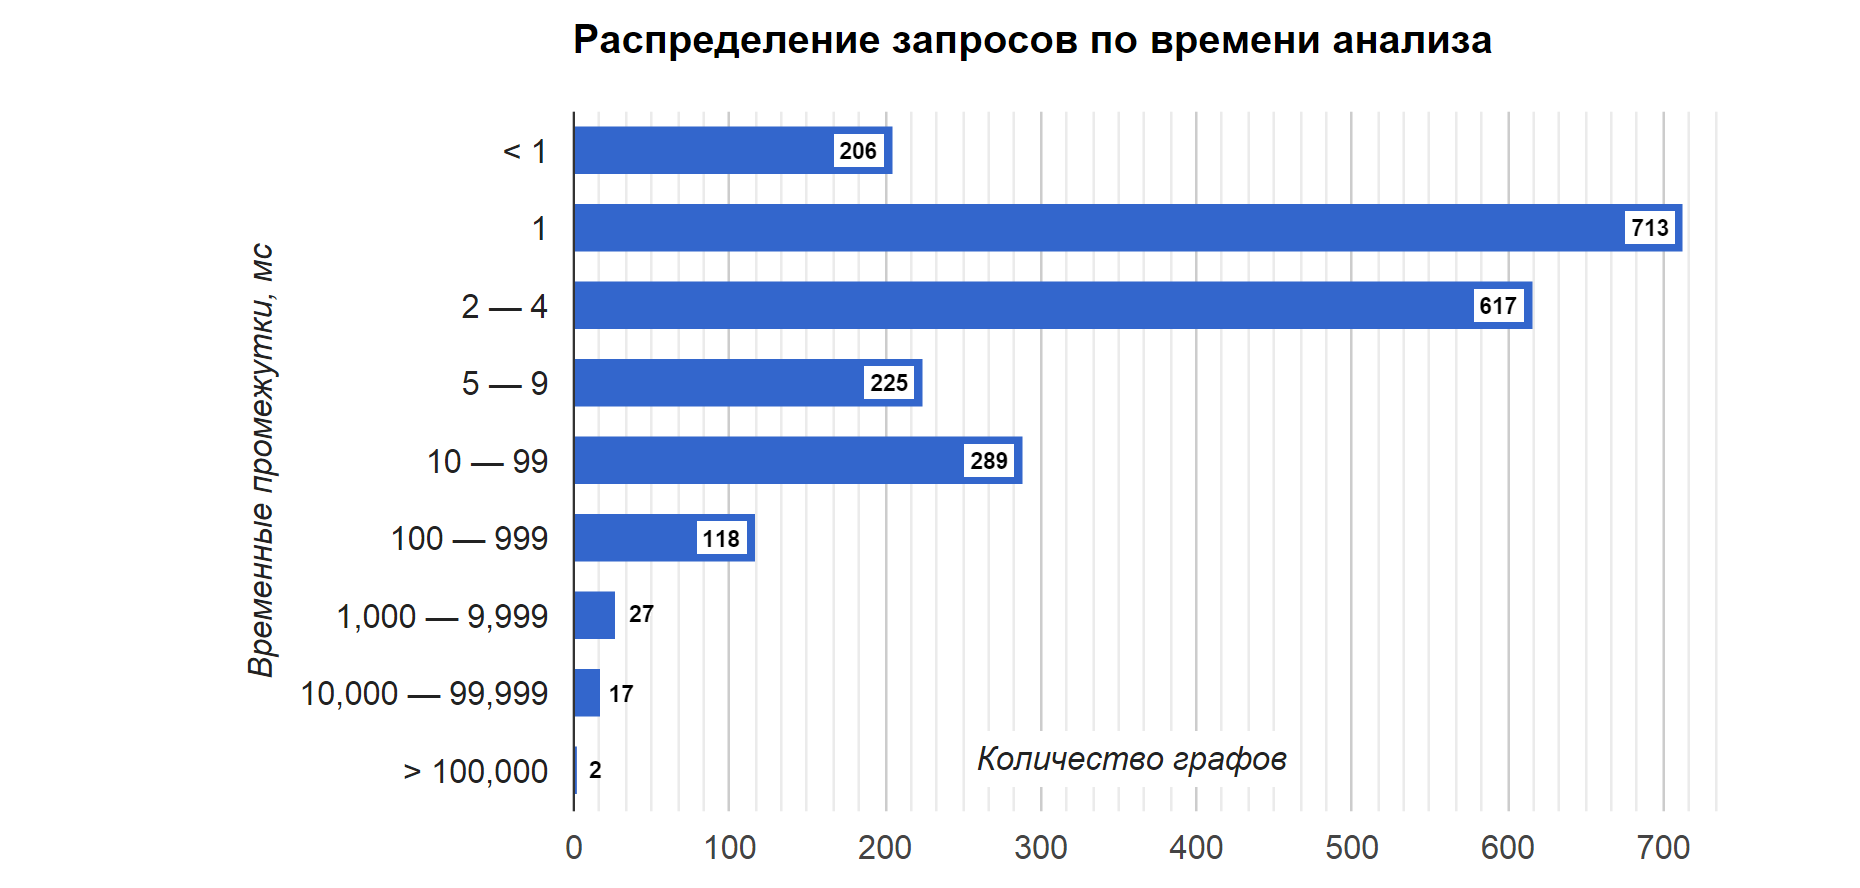
\includegraphics[width=10cm]{pictures/dist.png}
\end{frame}


\begin{frame}
  \transwipe[direction=90]
  \frametitle{Результаты}
  \begin{itemize}
    \item Разработан алгоритм синтаксического анализа регулярной аппроксимации динамически формируемых строковых выражений, строящий конечное представление леса разбора
    \item Доказана завершаемость и корректность алгоритма
    \item Выполнена реализация алгоритма на языке программирования F\# в рамках исследовательского проекта YaccConstructor
    \item Проведена апробация
  \end{itemize}

  \begin{itemize}
    \item Подана статья ``Relaxed Parsing of Regular Approximations of String-Embedded Languages'' на конференцию PSI-2015
  \end{itemize}
\end{frame}

\end{document}
